\PassOptionsToPackage{table}{xcolor}
\documentclass{cernatsnote}
\usepackage[colorinlistoftodos]{todonotes}
\usepackage{placeins}
\usepackage{float}
\usepackage{rotating}
\usepackage{pdflscape}
\usepackage{verbatim}
\usepackage{fancyvrb}
\usepackage{listings}
\usepackage[T1]{fontenc}
\usepackage{graphicx}
\graphicspath{{images/}}
\usepackage{xcolor}
\usepackage{colortbl}
\usepackage{booktabs}
\usepackage{longtable}
\usepackage{multirow}
\usepackage{array}
\usepackage{listings}
\lstdefinestyle{python}{
  language=Python,
  basicstyle=\small\ttfamily,
  keywordstyle=\color[RGB]{0,0,200}\bfseries,
  stringstyle=\color[RGB]{163,21,21},
  commentstyle=\color[RGB]{0,128,0}\itshape,
  numberstyle=\tiny\color{gray},
  frame=single,
  framerule=0.4pt,
  showstringspaces=false,
  breaklines=true,
  morekeywords={True,False,None},
}

\title{DFX4ML-ARCH (Progress Update 19-5-26)}
\author{
	Omitted for blind review \\
	CERN, CH-1211 Geneva, Switzerland
}
\email{Tanawin1701d@outlook.com}
\date{\today}

\begin{document}
\maketitle
 
\begin{abstract}
\end{abstract}

\tableofcontents

\pagebreak

\section{Architecture Upgrade}

A major refactor has been applied to almost all sections. The updated documentation is at \texttt{doc/tech\_report\_v0.2.pdf}.

\section{Barebone Testing}

\subsection{Hardware Setup}

We test with two reconfigurable regions, each containing a single reconfigurable module. The configuration used for the build is shown below.

\begin{lstlisting}[style=python]
from lib.hw_build import HwBuildHelper
from lib.sw_build import SwBuildHelper

board_build_tcl = "./kv260/board_build.tcl"
constraint_xdc  = "./kv260/constraint.xdc"

# Streamers (idx 0 = DMA)
dfx_streamers = [
    {"load_width": 4, "store_width": 4, 
	"actual_width": 32, "amount_row": 1024},  # s0
    {"load_width": 4, "store_width": 4, 
	"actual_width": 32, "amount_row": 1024},  # s1
]

# Regions: DMA -> r0 -> r1 -> DMA
dfx_regions = [
    {"load_streamers": [0], "store_streamers": [1]},  # r0
    {"load_streamers": [1], "store_streamers": [0]},  # r1
]

# RM schematics: rm_schemetics[region][rm]
rm_schemetics = [
    [{"load_io_map": [(0, 0)], "store_io_map": [(1, 0)]},],# r0 rm0
    [{"load_io_map": [(1, 0)], "store_io_map": [(0, 0)]},] # r1 rm0
]

hw_builder = HwBuildHelper(
    build_folder_path="./build_prj",
    dfx_root_path="../..",
    board="custom",
    board_build_tcl=board_build_tcl,
    constraint_xdc=constraint_xdc,
    user_repo_path="",
    user_rm_build_tcl_path="",
    req_gen_ip=1,
    num_core=4,
    clk_frq=99999001,           # Hz
    rm_index_width=2,           # max slots = 1 << width
    dfx_streamers=dfx_streamers,
    dfx_regions=dfx_regions,
    rm_schemetics=rm_schemetics,
    test_mode=1,
    vivado_path="/tools/Xilinx/Vivado/2023.2/bin/vivado",
    export_folder_path="./export"
)

hw_builder.run_build()
hw_builder.package_export_files()

sw_builder = SwBuildHelper(
    export_folder_path="./export",
    num_pr_region=2,
    rm_index_width=2,
    num_streamer=2,
)
sw_builder.package_export_file()
\end{lstlisting}

The resulting block design, built from the configuration listing above, is shown in Fig.~\ref{fig:block_design}. The internal hierarchies of \texttt{dfx\_unified} and \texttt{dma\_hier} are shown in Fig.~\ref{fig:dfx_unified} and Fig.~\ref{fig:dma_hier}, respectively.
 
\begin{figure}[H]
  \centering
  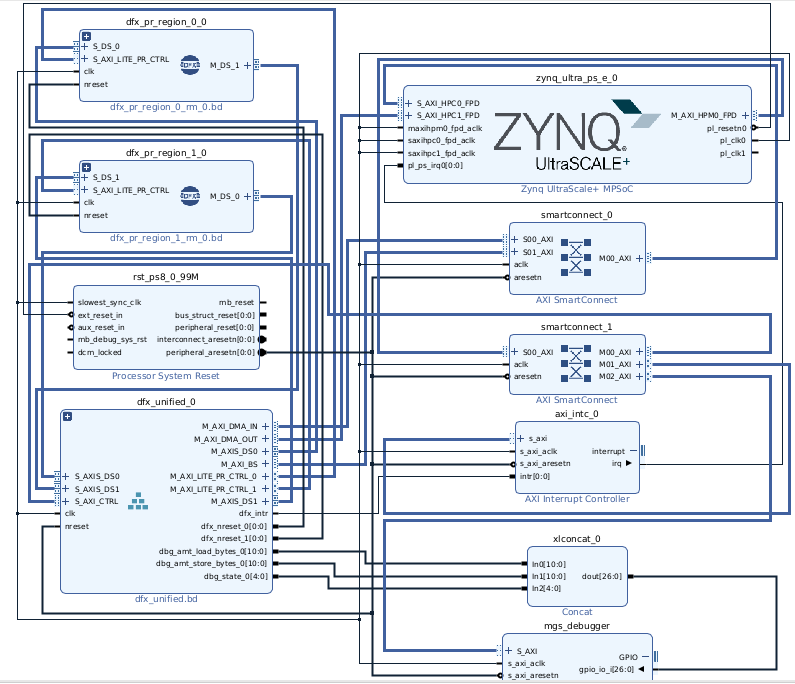
\includegraphics[width=0.95\linewidth]{block_design.png}
  \caption{Block design of the multi-region test setup.}
  \label{fig:block_design}
\end{figure}

\begin{figure}[H]
  \centering
  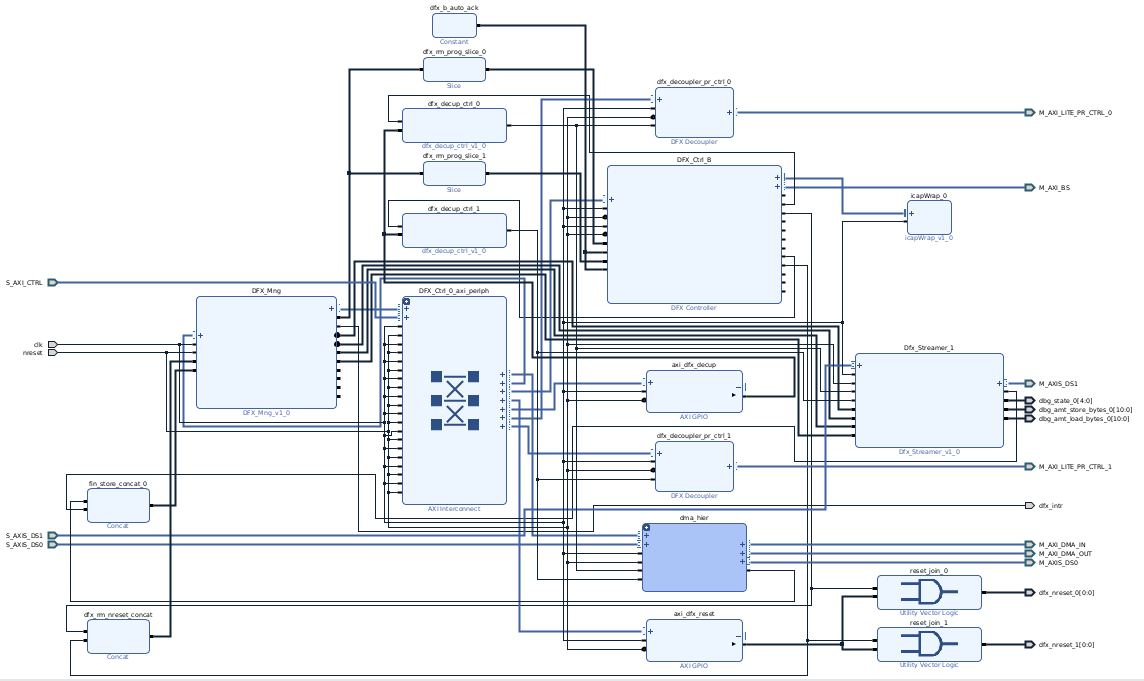
\includegraphics[width=0.95\linewidth]{dfx_unfied.png}
  \caption{\texttt{dfx\_unified} hierarchy.}
  \label{fig:dfx_unified}
\end{figure}

\begin{figure}[H]
  \centering
  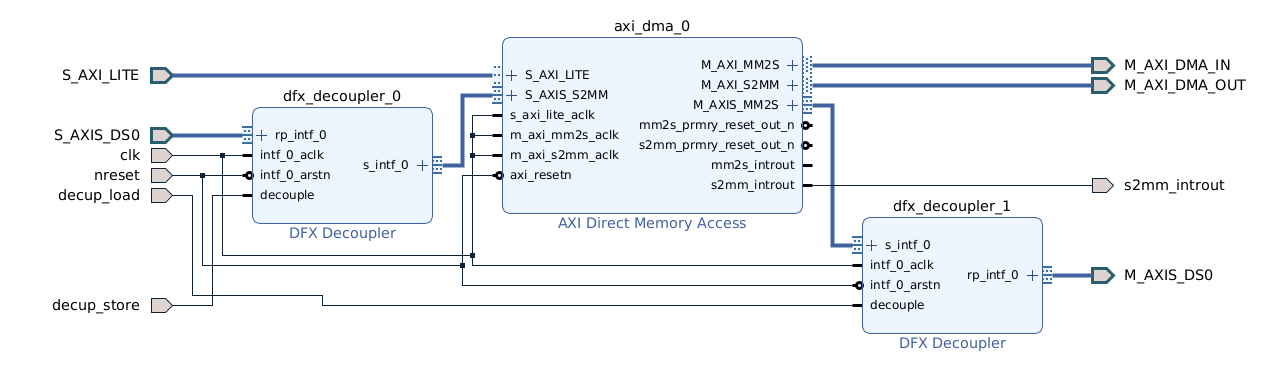
\includegraphics[width=0.95\linewidth]{dma_heir.png}
  \caption{\texttt{dma\_hier} hierarchy.}
  \label{fig:dma_hier}
\end{figure}


\subsection{Session Setup}

To orchestrate the flow, we use three sessions to support parallel execution:

\begin{itemize}
  \item \textbf{First session:} reconfigure region~0.
  \item \textbf{Second session:} execute data on region~0 (DMA $\rightarrow$ magic streamer~1), while reconfiguring region~1.
  \item \textbf{Final session:} execute data on region~1 (magic streamer~1 $\rightarrow$ DMA).
\end{itemize}

\begin{lstlisting}[style=python]
# Slot 0: recon only
dfx_mng.set_whole_slot(0, [
    0   ,      0, # src (none)
    0   ,      0, # dst (none)
    0   ,      0, # profile counters
    0b01,   0b00, # RM select (recon) (exec) (RM 0)
    0   ,      0, # load mask (none), store mask (ch0)
    0   ,         # complete mask
    1   ,         # next_session -> slot 1
])

# Slot 1: DMA-load input, execute with RM 0, no store yet
dfx_mng.set_whole_slot(1, [
    buf_input_phya, buf_input_sz,   # src
    0   ,    0   ,   # dst (none)
    0   ,    0   ,   # profile counters
    0b10, 0b01   ,   # RM select for recon / exec (RM 0)
    0b01, 0b10   ,   # load mask (ch0), store mask (none)
    0   ,            # complete mask
    2   ,            # next_session -> slot 2
])

# Slot 2: no load, execute with RM 0, DMA-store output -> wrap back to slot 0
dfx_mng.set_whole_slot(2, [
    0          ,              0, # src (none)
    buf_out_phy,     buf_out_sz, # dst
    0          ,              0, # profile counters
    0b00       ,           0b10, # RM select (RM 0)
    0b10       ,           0b01, # load mask (none), store mask (ch0)
    0          ,                 # complete mask
    0          ,                 # next_session -> slot 0 (wrap)
])
\end{lstlisting}

\subsection{Execution Result}

An example run of the three-session orchestration is shown in Fig.~\ref{fig:run_example}.

\begin{figure}[H]
  \centering
  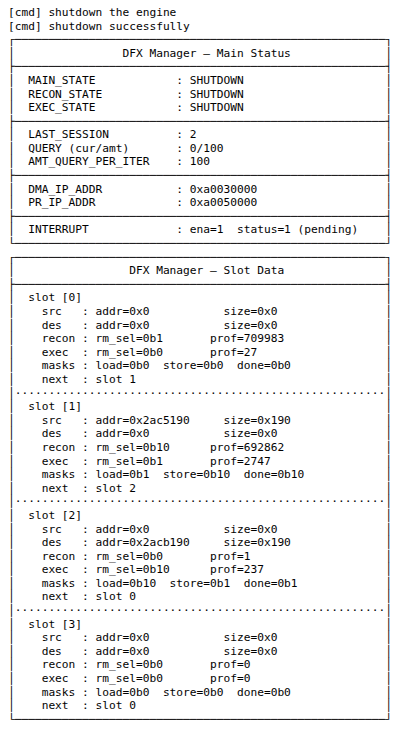
\includegraphics[width=0.8\linewidth]{run_exaxmple.png}
  \caption{Example run of the three-session orchestration.}
  \label{fig:run_example}
\end{figure}


\section{What's Next}

\begin{enumerate}
  \item We will perform further testing with dummy workloads, using multiple reconfigurable modules in each region.
  \item We will also test the synthetic ML workload from HLS4ML into DFX4ML.
\end{enumerate}


\end{document}
 